%!TEX root = /Users/oroce/Documents/msc-szakdolgozat/dolgozat.tex
A folyamatos integrációnál mivel naponta több verzió is kikerülhet, sőt párhuzamosan akár több csapat vagy akár fejlesztő is élesíthet funkciókat, ezért nagyon fontos, hogy a rendszer folyamatosan tájékoztassa a csapatokat az élesített funkciók működéséről hibáiról illetve a többiek által fejlesztett funkciók állapotáról. Mindehhez két dologra van szükség, a kommunikáció és a rendszer minden apró részének monitorozására, mert ezáltal a hibák gyorsan kiszűrhetőek, a reakció idő csökkenthető és mindenki valós időben láthatja, hogy mi történik a rendszerben, azaz transzparens lesz, amelynek köszönhetően a szervezetnek könnyebb a részegységek megismerése, felelősségi köreik meghatározása, megismerése.

\section{Chat rendszer}
A fejlesztői csapatok illetve a csapattagok közti kommunikáció rendkívül fontos, mely persze történhet verbálisan, azonban ez megszakíthatja a munkát, illetve távoli munkavégzés esetén (főleg ha a résztvevők más országból végzik a munkát) akkor sokkal jobb megoldás egy chatrendszer bevezetése, ilyenek lehetnek például:
\begin{itemize}
	\item Jabber\nomenclature{Jabber}{TODO}
	\item IRC\nomenclature{IRC}{IRC - Internet Relay Protocol}
	\item HipChat
	\item Campfire
	\item Grove.io
	\item FlowDock
\end{itemize}

\begin{table}
	\caption{Chat rendszerek összehasonlítása}[h]
	\begin{tabular}{ c | c | c | c | c | c | c }
	- & Jabber & IRC & HipChat & Campfire & Grove.io & FlowDock \\
	\hline
			Saját szerver & \ding{51} & \ding{51} & \ding{55} & \ding{55} & \ding{55} & \ding{55} \\
			Mobil alkalmazás & \ding{51} & \ding{51} & \ding{51} & \ding{55} & \ding{51} & \ding{55} \\
			Asztali alkalmazás & \ding{51} & \ding{51} & \ding{51} & \ding{55} & \ding{55} & \ding{55} \\
			Egy-az-egy beszélgetés & \ding{51} & \ding{51} & \ding{51} & \ding{55} & \ding{55} & \ding{55} \\
			Csoportbeszélgetés & \ding{51} & \ding{51} & \ding{51} & \ding{55} & \ding{55} & \ding{55} \\
			Audió, Videó & \ding{51} & \ding{51} & \ding{51} & \ding{55} & \ding{55} & \ding{55} \\
			Email értesítés & \ding{51} & \ding{51} & \ding{51} & \ding{55} & \ding{55} & \ding{55} \\
	\hline
	\multicolumn{7}{l}{Forrás: \cite{chat_compare_hipchat}, \cite{chat_compare_campfire}, \cite{chat_compare_grove}, \cite{chat_compare_flowdock}}
	\end{tabular}
\end{table}
De miért kell chat, miért nem elég az email alapú kommunikáció?\\
\hfill\\
A legtöbb szervezetben sajnos még mindig az email a legfontosabb kommunikációs eszköz, azonban az email lassú, nem alkalmas instant üzenetek küldésére, illetve gyakran kimaradnak a levelezésből megfelelő emberek, ezzel ellentétben viszont a cseten gyorsan lehet üzenetet váltani. Természetesen a csettel nem lehet kiváltani az emailt, a két eszközt kombinálva, egymást segítve lehet jól használni.
Továbbá a cset mellett érvelve elmondható, hogy az emberek könnyebben elviselik a zajt csetet használva, mint az emailezésben.\textbf{}

\section{Naplózás, naplógyűjtés\\}

Az alkalmazások viselkedésének monitorozása rendkívül fontos, ugyanis amint kikerülnek a belső homokozóból, akkor megváltozhatnak a reakcióik a felhasználók különbőző tevékenységeire, ezeknek a problémák a felderítése használják a naplózás és a naplógyűjtést. Érdemes kiemelni, hogy a fejlesztési (development), tesztelési (staging/user acceptence testing) illetve az előnézeti (preview) szerverek is mind valamilyen homokozónak számítanak, hiszen valós felhasználók nem használják, a felhasználók szimulálása - akár tesztelők, akár automatizált tesztek által - szinte sosem tökéletesek.
\\
A jól használt naplózással a hibák hamarabb kiszűrhetőek, a hibák forrása könnyebben kiszűrhető, azonban minden rendszer naplójainak egyidejű figyelése egyszerűen lehetetlen. Ezért használnak a legtöbb rendszerben központi naplózást és naplógyűjtést, amelynek segítségével a hibák felfedezése, forrásának felderítése és a megoldása is könnyebben megoldható. Miért lehetne a központi naplózással könnyebben megoldani egy problémát? Amennyiben az alkalmazás példánya tegyük fel lassan válaszol, miközben a többi példány hiba nélkül működik (ezt egy könnyű ellenőrizni, hiszen egymás mellé helyezhető az alkalmazás példányok naplója), akkor egyértelmű, hogy a hiba a példányt futtató eszközön van csak jelen - a legtöbb esetben - amely megkönnyíti a szakembereknek a hibajelenség elhárítását.
\\
Továbbá a központi naplózás könnyen implementálható a folyamatos értesítés munkafolyamataiba, amellyel egy-egy alkalmazás/termék felelős szakembere azonnal értesülhet a fenálló hibáról, a javítást azonnal elkezdheti.
\\ 
A piacon több naplógyűjtő alkalmazás is elérhető mind telepíthető, mind \nomenclature{SaaS}{TODO} formában. A telepíthető és SaaS verzióban is elérhető többet a között a \emph{GrayLog2}.
\\
\subsection{GrayLog2}
A GrayLog2 segítségével könnyen monitorozható az összes szoftveres hiba, legyen szó akár adatbázisról, az operációs rendszer hibáiról vagy alkalmazáshibáról. Emelett lehetőséget nyújt nem csak hibajellegű üzenetek tárolására, hanem a hibakereséshez szükséges üzenetek megjelenítésére is.

\begin{figure}[ht]
	\centering
		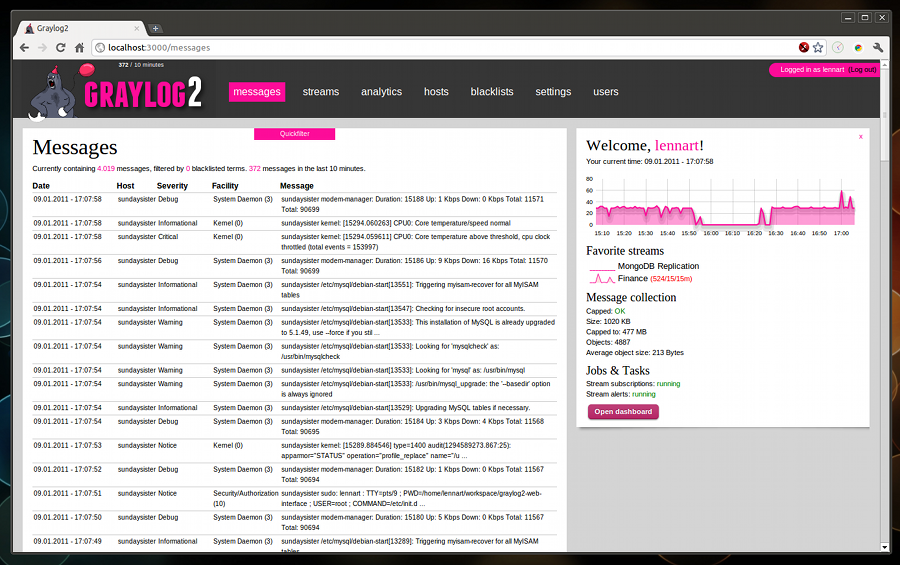
\includegraphics[scale=0.5]{assets/graylog2.png}%
		\caption[DUMMY]%
		{A GrayLog2 interfésze}%
		\label{fig:graylog2-webinterface}
\end{figure}

\Aref{fig:graylog2-webinterface} ábrán látható a GrayLog2 webes interfésze, amelynek segítségével a szakemberek könnyen észlelhetik valós időben a fennálló vagy éppen bekövetkező hibákat, továbbá kereshetnek a korábban előforduló hibákban (erre a GrayLog2 az \nomenclature{ElasticSearch}{TODO} \nomenclature{full-text search engine}{TODO} szoftvert használja) illetve könnyen beállíthatnak értesítéseket, hogy akár az éjszaka felmerülő hibákról is értesülhessen a felelős.

\section{Alkalmazás hiba monitorozás\\}
A naplózással a hibák könnyen észrevehetővé és később visszakereshető válnak, azonban a következőkre nem nyújt megoldást:\\
\begin{itemize}
\item hibák rögzítése a jegykezelő (issue kezelő) rendszerben
\item egy hiba csak egyszer kerüljön rögzítésre
\item automatikus értesítés a hibáról
\item a hibászázalék vizualizálása komponensenként
\end{itemize}

Természetesen alkalmazás hiba monitorozó rendszer nélkül is működhet rendszer jól, azonban előfordulhat, hogy nagy mennyiségű hibánál a naplógyűjtő rendszerben átsiklanak problémák felett vagy egyszerűen elfelejtésre kerülnek. A másik probléma lehet amikor a hibajelentést közvetlenül a jegykezelő rendszerbe kötik be. Ez miért lehet probléma? Egy nagy felhasználóbázissal rendelkező rendszernél, ha hiba csak a felhasználók néhány százalékánál fordul elő, akkor is szükségtelenül nagy mennyiségű jegy keletkezést fogja előidézni.\\

Az alkalmazás hiba monitorozás leginkább a nem webes alkalmazásoknál (mobil és asztali) terjedt el az utóbbi időben, ugyanis ezeknél a rendszereknél a naplók nem, vagy csak nehezen gyűjthetők valós időben.\\

Elérhető alkalmazások:
\begin{itemize}
\item Sentry - \url{http://getsentry.com}
\item Exceptional - \url{http://www.exceptional.io/}
\item Bugsense - \url{http://www.bugsense.com/}
\end{itemize}

\begin{figure}[ht]
	\centering
		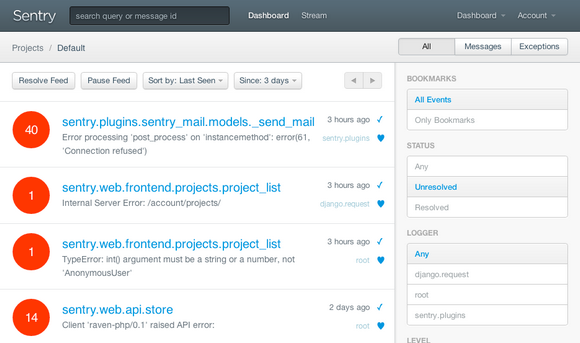
\includegraphics[scale=1]{assets/sentry.png}%
		\caption[DUMMY]%
		{A Sentry interfésze}%
		\label{fig:sentry}
\end{figure}

\section{Szolgáltatások integrálása\\}

A fejezetben említett említett szolgáltatás, szoftverek használatával a fejlesztők, adminisztrátorok már jobban megismerhetik saját alkalmazásikat, azonban ennyi felület, értesítés nyomon követése szinte már lehetetlen, ezért minden szervezet próbálja ezeket az eszközöket egymásba integrálni.
\begin{figure}[ht]
	\centering
		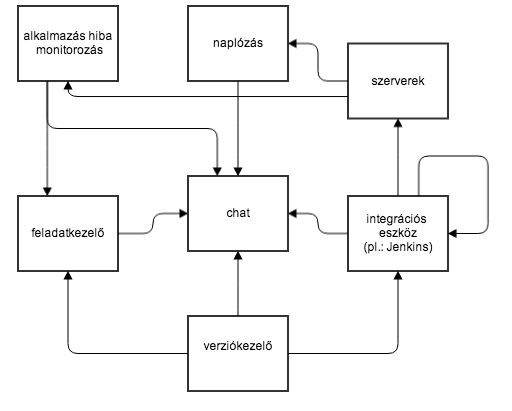
\includegraphics[scale=1.0]{assets/integrated_services.png}%
		\caption[DUMMY]%
		{A szolgáltatások egy lehetséges integrálása}%
		\label{fig:integrated-services}
\end{figure}
\Aref{fig:integrated-services} ábrán látható a szolgáltatások egy lehetséges integrációja. Első ránézésre az ábra bonyolultnak és összetettnek tűnhet, mert sok különböző egység integrációját igényli emellett a részegységeknek valós időben kell kommunikálniuk, tudniuk kell a sorrendet, és képeseknek kell lenniük egymás üzeneteinek megértésére.\\
Ezeknek az igénynek a kielégítésére minden részegység tudja, hogy kit kell neki értesítenie; az értesítések pedig ún. \emph{webhook} (\cite{web_hook}) használatával történik, amely egy egyszerű HTTP kérés, ezáltal valós időben történhet meg az következő részegység notifikálása.\\
Viszont hogyan képesek megérteni egymás üzeneteit a részegységek?\\
Erre sajnos nincs sztenderd specifikáció, azonban szinte minden említett eszköz nyílt forrású és széles körben elterjedt, ezért egymás üzeneteinek feldolgozása, megértése már megoldott beépülők használatával.\\

\Aref{fig:integrated-services} ábrán felrajzolt folyamatnak az első szintje az amikor a kód bekerül a verziókezelőbe, amely össze van kapcsolva a feladatkezelővel, ahol akár a kapcsoló jegy lezárásra is kerülhet a kód mellé csatolt üzenet szövege (\nomenclature{commit message}{TODO}) alapján, majd a chaten keresztül értesülhetnek a csapat tagjai, a projektmenedzser vagy az adott szervezeten belül bárki, aki érintett lehet az adott funkció, szolgáltatás fejlesztésében.\\
A verziókezelő másik kapcsolata az integrációs eszközzel van, amely lefuttat különböző ellenőrző, tesztelési és riportálási feladatokat, amelyek garantálják, hogy az új kódsorok megfelelnek a céges előírásoknak, nem okoznak problémát az alkalmazás futtatásában, a folyamat végén értesítést küldhet a közös chatbe az integráció sikerességéről, hiba esetén értesítheti a megfelelő személyeket, ugyanis a hiba kijavításáig senki tud hibámentes kódot beküldeni az integrációs folyamatba, ezért ennek az értesíthet a legmagasabb prioritással kell történnie. Az integrációs folyamat kimenete lehetséges, hogy újabb integrációs folyamat bemenete lesz; ez olyankor fordulhat elő, amikor az alkalmazás egyik ága egy másik ágba kerül beolvasztásra. Ez történhet például a fejlesztői ág tesztelői ágba való automatikus vagy félautomatikus olvasztásakor, vagy a minőségbiztosítási csapat (\nomenclature{QA team}{TODO}) tesztelői ág jóváhagyásaként a produkciós ágba való olvasztáskor.\\
\hfill\\
\Aref{fig:integrated-services} ábrán továbbhaladva az integrációs eszköz után az alkalmazás felhasználói elfogadási szerver (user acceptance test server) vagy előnézeti (staging, preview) szerverre kerül, amely egy homokozószerű, zárt, a produkciós szerverrel megegyező architektúrájú környezetben nyújt lehetőséget az alkalmazás tesztelésére. Majd ezután kerülhet ki a produkciós szerverre. Mind a felhasználói elfogadási, az előnézeti és a produkciós szerverek hibáit már naplózni illetve az ezeken futó alkalmazásokét is; hiba esetén pedig értesíteni kell a chaten keresztül az hibát okozó komponens, vagy alkalmazás részért felelős személyt, csapatot. A felelősök a hibáról hibajegyet készíthetnek a feladatkezelőbe, majd a fejlesztőcsapatok javítva a hibát a kódot beküldik a verziókezelőbe és a folyamat újraindul.\\
\hfill\\
Fontos felhívni a figyelmet, hogy \aref{fig:integrated-services} ábrán rendkívül komoly hangsúlyt kapott a chat rendszer, természeten nem kötelező csetet használni, azonban a valós idejű értesítésekre illetve a reakcióidő csökkentése érdekében mindenképpen ajánlott. Továbbá az ábrán nem szerepel, de a cset alapú notifikálás mellett érdemes egy értesítése formákat is használni, mint például az email, vagy magas prioritású hibáknál (alkalmazásleállás) érdemes lehet megfontolni az sms, okostelefon valós idejű üzenet (\nomenclature{Push Notification}{TODO}), esetleg csipogó használatát.

\subsection{Hubot}
Ha egy szervezet úgy dönt, hogy csetet fog használni a rendszerek, alkalmazások valós idejű követésére, akkor találkozni fog a következő problémákkal:
\begin{description}
\item[Rendszerautomatizáció] hiába automatizált a folyamat, ha az egy-egy pontról történő elindítás nem lehetséges, bárhonnan, bármikor.\\
Ilyen probléma lehet az integrációs rendszer elindítása a kód egy pillanatnyi állapotától kód beküldés nélkül.
\item[Távoli irányítás] lehet, hogy egy asztali számítógépen könnyen elvégezhető a produkciós rendszeren egy verzióváltás, de miért ne lehetne ezt megtenni egy okostelefonról is?
\item[Kommunikáció külső eszközök használatakor] ha egy üzenet érkezik (például alkalmazás újraindítás szükségességéről), akkor a csapat tagjainak meg kell beszélniük, hogy ki javítja meg a problémát.
\end{description}
GitHub, Inc., wrote the first version of Hubot to automate our company chat room. Hubot knew how to deploy the site, automate a lot of tasks, and be a source of fun in the company. Eventually he grew to become a formidable force in GitHub. But he led a private, messy life. So we rewrote him.

Today's version of Hubot is open source, written in CoffeeScript on Node.js, and easily deployed on platforms like Heroku. More importantly, Hubot is a standardized way to share scripts between everyone's robots.